\documentclass{article}
\usepackage[utf8]{inputenc}
\usepackage{amsmath}
\usepackage{graphicx}
\graphicspath{ {./images/} }
\usepackage{hyperref}

\title{RL Excercise Chapter 2}
\author{huseyinabanox }
\date{June 2022}

\begin{document}

    \maketitle
    \setcounter{section}{1}


    \section{Exercises}

    \subsection{Question}
    In \(\epsilon\)-greedy action selection, for the case of two actions and \(\epsilon = 0.5 \), what is the probability that the greedy action is selected?

    \subsection*{Answer}

    Greedy action is selected with a probability of $0.5$. Greedy action can also be selected in random action selection with a probability of $(1-\epsilon)*0.5 = 0.5 * 0.5 = 0.25 $
    Overal probability is $ 0.5 + 0.25 = 0.75 $

    \subsection{Question}

    Consider a k -armed bandit problem with k = 4 actions,
    denoted 1, 2, 3, and 4. Consider applying to this problem a bandit algorithm using
    $\epsilon-$greedy action selection, sample-average action-value estimates, and initial estimates
    of Q 1 (a) = 0, for all a. Suppose the initial sequence of actions and rewards is A 1 = 1,
    R 1 = 1, A 2 = 2, R 2 = 1, A 3 = 2, R 3 = 2, A 4 = 2, R 4 = 2, A 5 = 3, R 5 = 0. On some
    of these time steps the $\epsilon$ case may have occurred, causing an action to be selected at
    random. On which time steps did this definitely occur? On which time steps could this
    possibly have occurred?

    \subsection*{Answer}

    \begin{table}[]
        \begin{tabular}{llllllll}
            t & Q(A1) & Q(A2) & Q(A3) & Greedy & Selected & Reward & Random?  \\
            0 & 0     & 0     & 0     & Any    & 1        & -1     & Probable \\
            1 & -1    & 0     & 0     & 2,3,4  & 2        & 1      & Probable \\
            2 & -1    & 1     & 0     & 2      & 2        & -2     & Probable \\
            3 & -1    & -1/2  & 0     & 3,4    & 2        & 2      & Yes      \\
            4 & -1    & 1/3   & 0     & 2      & 3        & 0      & Yes      \\
        \end{tabular}
    \end{table}

    Random action selection may result in the selection of greedy action.
    Thus all steps may involve random action selection.

    If greedy action and selected actions are different then random selection is certain.

    \subsection{Question}

    In the comparison shown in Figure 2.2, which method will perform best in the long run in
    terms of cumulative reward and probability of selecting the best action? How much better will it be?
    Express your answer quantitatively.

    \subsection*{Answer}

    In the long run optimal action a* is found.
    Even after finding optimal action, $\epsilon-$greedy method will continue exploring.

    \textbf{Optimal action selection:}

    Optimal action is selected with probability $1-\epsilon$.
    Non-optimal action is selected with probability $\epsilon$.
    Optimal action a* may be selected randomly with a probability $\epsilon/k$.
    k is given as 10.

    Total probability of selecting the optimal action is:

    \begin{equation}
        P(A_i=a^*) = 1-\epsilon + \epsilon/10
    \end{equation}

    Considering given $\epsilon$ values:

    \begin{equation}
        \frac{P(A_i=a^*|\epsilon=0.01 ) }{P(A_i=a^*|\epsilon=0.1 ) }= \frac{1-0.01 + 0.01/10}{1-0.1 + 0.1/10} = 0.991 /0.91 = 1.09
    \end{equation}

    \textbf{Average reward:}

    Since they are derived from the same distributed with a mean of 0, expected value of all actions combined is 0.
    Thus average reward for random actions will be zero.
    We will only consider average reward for greedy action selections.

    In the long run average reward will be equal to expected value of selecting greedy action:

    \begin{equation}
        E[R]=q^*(a^*)*(1-\epsilon)
    \end{equation}

    Considering given $\epsilon$ values:

    \begin{equation}
        \frac{E[R|\epsilon=0.01]}{E[R|\epsilon=0.1]} = \frac{q^*(a^*)*(1-0.01)}{q^*(a^*)*(1-0.1)} = \frac{0.99}{0.9} = 1.1
    \end{equation}

    \subsection{Question}
    f the step-size parameters, \(\alpha_n\), are not constant, then the estimate \(Q_n\) is a weighted
    average of previously received rewards with a weighting different from that given by (2.6). What is
    the weighting on each prior reward for the general case, analogous to (2.6), in terms of the sequence of
    step-size parameters?

    \subsection*{Answer}

    \begin{equation}
        Q_{n+1}=Q_{n}+\alpha_{n}[R_n-Q_n]=\alpha_{n}R_n+(1-\alpha_{n})Q_n
    \end{equation}

    \begin{equation}
        Q_{n+1}=\alpha_{n}R_n+(1-\alpha_{n})[Q_{n-1}+\alpha_{n-1}[R_{n-1}-Q_{n-1}]]=\alpha_{n}R_n+(1-\alpha_{n})[\alpha_{n-1}R_{n-1}+(1-\alpha_{n-1})Q_{n-1}]
    \end{equation}

    \begin{equation}
        Q_{n+1}=\alpha_{n}R_n+(1-\alpha_{n})\alpha_{n-1}R_{n-1}+ (1-\alpha_{n}) (1-\alpha_{n-1})Q_{n-1}
    \end{equation}

    \begin{equation}
        Q_{n+1}=\alpha_{n}R_n+(1-\alpha_{n})\alpha_{n-1}R_{n-1}+ (1-\alpha_{n}) (1-\alpha_{n-1})[\alpha_{n-2}R_{n-2}+(1-\alpha_{n-2})Q_{n-2}]
    \end{equation}

    \begin{equation}
        Q_{n+1}=\alpha_{n}R_n+(1-\alpha_{n})\alpha_{n-1}R_{n-1}+ (1-\alpha_{n}) (1-\alpha_{n-1})\alpha_{n-2}R_{n-2}+(1-\alpha_{n}) (1-\alpha_{n-1})(1-\alpha_{n-2})Q_{n-2}
    \end{equation}

    \begin{equation}
        Q_{n+1}=\sum_{i=0}^{n-1} \alpha_{n-i}R_{n-i} \prod_{k=0}^{i-1}(1-\alpha_{n-k}) + Q_1 \prod_{i=0}^{n-1}(1-\alpha_{n-i})
    \end{equation}

    \subsection{Question}

    In the comparison shown in Figure 2.2, which method will perform best in the long run in
    terms of cumulative reward and probability of selecting the best action? How much better will it be?
    Express your answer quantitatively.

    \subsection*{Answer}
    A modified version of the 10-armed testbed from \href{https://github.com/LyWangPX/Reinforcement-Learning-2nd-Edition-by-Sutton-Exercise-Solutions}{https://github.com/LyWangPX} is used.

    First two bandits do not make random walk. Last two bandits make random walk.

    Constant step size performs better in case of random walk which creates a non-stationary target.

    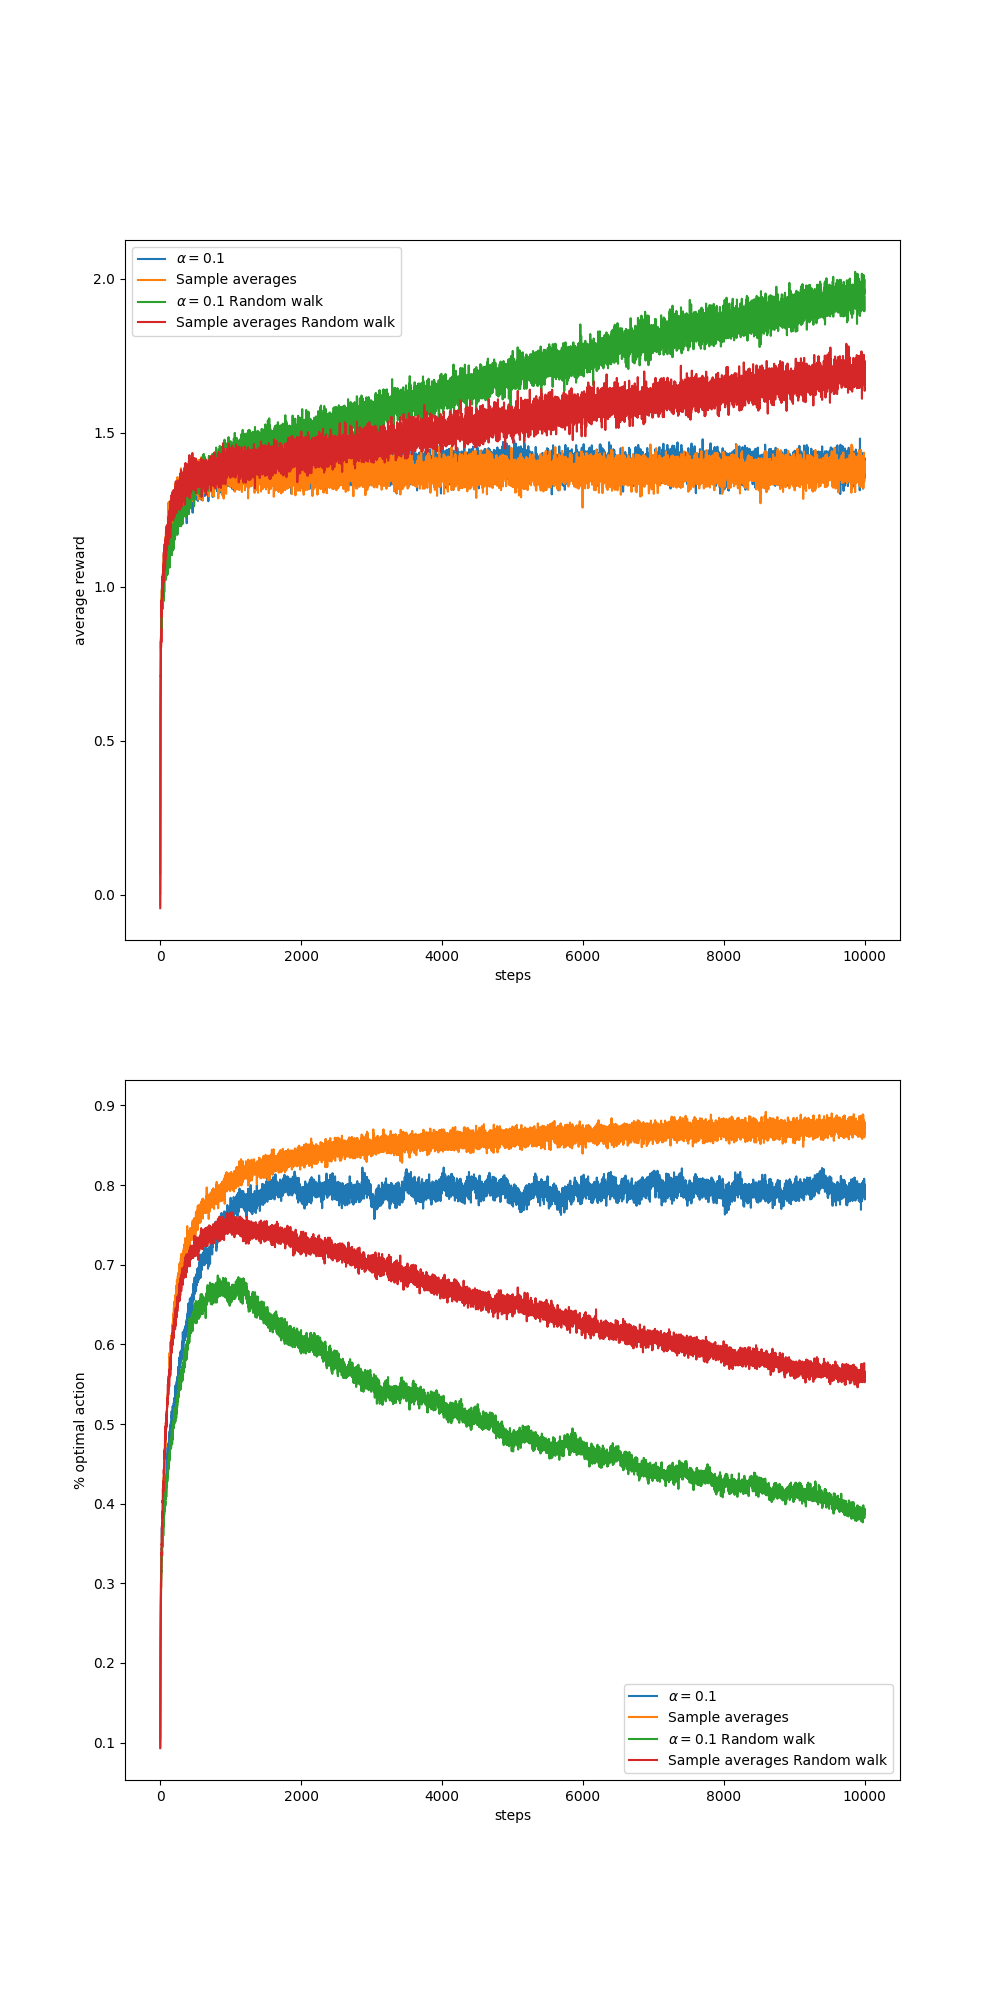
\includegraphics[scale=0.5]{figure_e_2_5}

    \subsection{Question}

    The results shown in Figure 2.3 should be quite reliable because
    they are averages over 2000 individual, randomly chosen 10-armed bandit tasks. Why, then, are there
    oscillations and spikes in the early part of the curve for the optimistic method? In other words, what
    might make this method perform particularly better or worse, on average, on particular early steps?

    \subsection*{Answer}

    Figure 2.3 shows optimal action selection behaviour.
    Optimistic initial value encourages exploration.
    Since all arms have equally optimistic high values, arms are selected randomly.
    Once the optimum action is selected its value is downgraded through the true value.
    In following few steps, non-optimal actions with higher value are selected.
    Non-optimal actions are downgraded faster than the optimal action.

    Optimistic strategy explores early and learns obtains a good view about the optimum behaviour.
    Even though it oscilates dramatically in the beginning it improves faster.
    Optimistic method stops exloring once actual values are learnt which is good only for stationary problems.

    Realistic method with $\epsilon-$greedy exploration explorer less frequent in the beginning thus learns more slowly.

    For non-stationary problems $\epsilon-$greedy performs better since it continues exploration even after initial stage.

    \subsection{Question}
    Is it possible to avoid the bias of constant step sizes while retaining their advantages on nonstationary problems? One way is to use a step size of ...
    Carry out an analysis like that in (2.6) to show that Qn is an exponential recency-weighted average without initial bias.

    \subsection*{Answer}
    $(1-\alpha)^{n}Q_1$ section in (2.6) carries the initial bias.
    With new method it becomes $(1-\beta_1)(1-\beta_2)(1-\beta_3)\ldots(1-\beta_n)Q_1$.

    As n gets larger, the trace parameter quickly approaches to 1.
    When it is close to 1, step size $\beta$ approaches to one and $(1-\beta)$ becomes very small and effectively eliminates the initial bias.

    \subsection{Question}
    UCB Spikes In Figure 2.4 the UCB algorithm shows a distinct spike
    in performance on the 11th step. Why is this? Note that for your answer to be fully
    satisfactory it must explain both why the reward increases on the 11th step and why it
    decreases on the subsequent steps. Hint: if c = 1, then the spike is less prominent.

    \subsection*{Answer}
    At start uncertainity on optimal action is high and UCB selects optimal actions. Then uncertainity becomes low and UCB prefers non-optimal actions.
    Updated optimal action values stop the curve going further down.

    \subsection{Question}
    Show that in the case of two actions, the soft-max distribution is the same as that given by the logistic, or sigmoid, function often used in statistics and artificial neural networks.

    \subsection*{Answer}
    \begin{equation}
        Pr(A_1=a)=\frac{e^{H_{1}(a)}}{ e^{H_{1}(a)}+e^{H_{1}(b)} } = \frac{1}{ 1+e^{H_{1}(b)-H_{1}(a)} } = sigmoid(H_{1}(a)-H_{1}(b))
    \end{equation}

    \subsection{Question}
    Suppose you face a 2-armed bandit task whose true action values change randomly from time step to time step.
    Specifically, suppose that, for any time step, the true values of actions 1 and 2 are respectively 0.1 and 0.2 with probability 0.5 (case A), and 0.9 and 0.8 with probability 0.5 (case B).
    If you are not able to tell which case you face at any step, what is the best expectation of success you can achieve and how should you behave to achieve it?
    Now suppose that on each step you are told whether you are facing case A or case B (although you still don’t know the true action values).
    This is an associative search task.
    What is the best expectation of success you can achieve in this task, and how should you behave to achieve it?

    \subsection*{Answer}

    Each case may occur with the same probability.

    $E[q]=E[q|A]+E[q|B]$

    \subsubsection*{Case not known}

    There is no way we can learn about the actual action values thus the best we can do is to select the arms uniformly and take the average reward for each arm.

    $E[q|1]=0.5*(0.2)+0.5*(0.8) = 0.5$

    $E[q|2]=0.5*(0.1)+0.5*(0.9) = 0.5$

    $E[q|A] = E[q|A,1] + E[q|A,2] = 0.5 * 0.5 + 0.5 * 0.5 = 0.5 $

    $E[q|B] = E[q|B,1] + E[q|B,2] = 0.5 * 0.5 + 0.5 * 0.5 = 0.5 $

    $E[q]=E[q|A]+E[q|B] = 0.5 * 0.5 + 0.5 * 0.5 = 0.5$

    \subsubsection*{Case known}

    Since cases are known, it is possible to learn action values for each arm in each case.
    Thus it becomes possible to act optimally in each case.

    $E[q|A, 1] = 0.1, E[q|A, 2] = 0.2$

    $E[q|B, 1] = 0.9, E[q|B, 2] = 0.8$

    It is optimal to select arm 2 in case A, it is optimal to select arm 1 in case B.

    $E[q|A] = E[q|A,2] = 0.2 $

    $E[q|B] = E[q|B,1] = 0.9 $

    $E[q]=E[q|A]+E[q|B] = 0.5 * 0.2 + 0.5 * 0.9 = 0.55$

    \subsection{Question}

    (programming) Make a figure analogous to Figure 2.6 for the nonstationary case outlined in Exercise 2.5. Include the constant-step-size "$\epsilon-$greedy algorithm with $\alpha$ = 0.1.
    Use runs of 200,000 steps and, as a performance measure for each algorithm and parameter setting, use the average reward over the last 100,000 steps.

    \subsection*{Answer}

    A modified version of the 10-armed testbed from \href{https://github.com/LyWangPX/Reinforcement-Learning-2nd-Edition-by-Sutton-Exercise-Solutions}{https://github.com/LyWangPX} is used.

    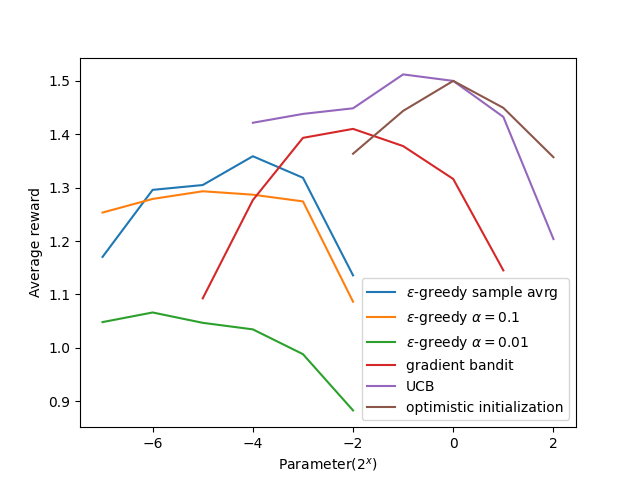
\includegraphics[scale=0.5]{figure_e_2_11}

\end{document}



